\documentclass{article}
\usepackage{tikz}

\begin{document}
\pagestyle{empty}

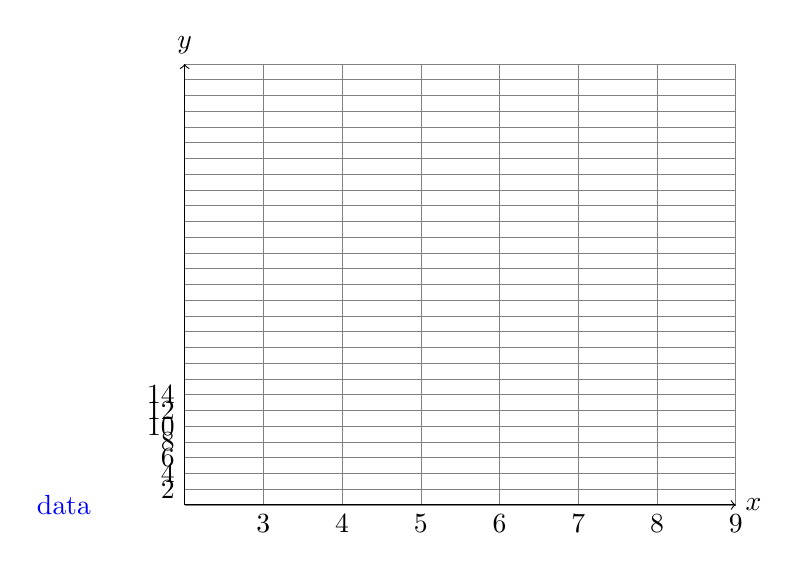
\begin{tikzpicture}[x=1cm,y=0.1cm]

  \def\xmin{2}
  \def\xmax{9}
  \def\ymin{0}
  \def\ymax{56}

  % grid
  \draw[style=help lines, ystep=2, xstep=1] (\xmin,\ymin) grid
  (\xmax,\ymax);

  % axes
  \draw[->] (\xmin,\ymin) -- (\xmax,\ymin) node[right] {$x$};
  \draw[->] (\xmin,\ymin) -- (\xmin,\ymax) node[above] {$y$};

  % xticks and yticks
  \foreach \x in {3,4,...,9}
    \node at (\x, \ymin) [below] {\x};
  \foreach \y in {2,4,...,14}
    \node at (\xmin,\y) [left] {\y};

  % plot the data from the file data.dat
  % smooth the curve and mark the data point with a dot
 
\draw[color=blue] plot[smooth] file {k.dat}
   node [right] {data};



\end{tikzpicture}

\end{document}
